\begin{ledgroupsized}[r]{120mm}
\footnotesize 
\pstart 
\noindent\textbf{\"{U}berlieferung:}
\pend
\end{ledgroupsized}
\begin{ledgroupsized}[r]{114mm}
\footnotesize 
\pstart \parindent -6mm
\makebox[6mm][l]{\textit{L}}%
Konzept: 
LH XXXV 10, 9 Bl. 3-4. 1 Bog. 2\textsuperscript{o}. 1\,\nicefrac{1}{2} S. auf Bl. 4.
Der Bogen überliefert ferner  N.~28\textsubscript{1}, N.~28\textsubscript{2}, N.~28\textsubscript{5} und N.~5.
%LH35,10,09 Bl. 3r = Demonstratio geometrica de magnetis sphaera
\\
Cc 2, Nr. 1192 A-B
\pend
\end{ledgroupsized}
%
%\vspace*{5mm}
%\begin{ledgroup}
%\footnotesize 
%\pstart
%\noindent\footnotesize{\textbf{Datierungsgr\"{u}nde}: nur chronologische Einordnung, Datierung nicht erfolgt}
%\pend
%\end{ledgroup}

\vspace*{8mm}
\pstart 
\normalsize
\noindent
[4~r\textsuperscript{o}] Determinata machinae vi\protect\index{Sachverzeichnis}{vis} per certam quandam relationem seu velut aequationem, ut hoc loco: \rule[-4mm]{0pt}{10mm}$\displaystyle\frac{ya + a \sqrt{a^2-y^2} - yb - b\sqrt{a^2-y^2}}{ba}$. 
\pend
\pstart
Hinc determinari potest vis\protect\index{Sachverzeichnis}{vis} ejus per accelerationem\protect\index{Sachverzeichnis}{acceleratio} acquisita. Nam regula generalis \makebox[1.0\textwidth][s]{est: sit figura $ABC$ cujus ordinatarum differentiae, $FG. HI. KB$, sint ut vires machinae\protect\index{Sachverzeichnis}{vires machinae}}
\pend
\vspace{1em}
\begin{minipage}[t]{0.5\textwidth}
%\hspace*{-5mm}
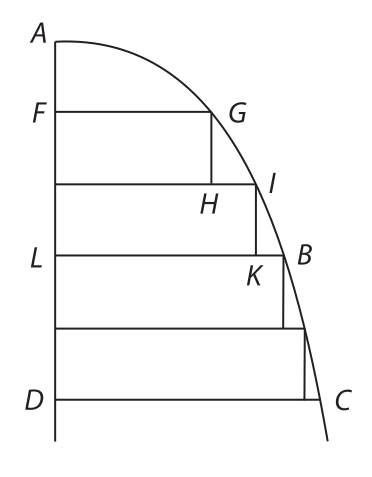
\includegraphics[width=0.65\textwidth]{images/lh0351009_004r-d1.pdf}
%\noindent \centering [\textit{Fig. 1}]
\end{minipage}
%\hspace*{17,3mm}
\begin{minipage}[t]{0.5\textwidth}
%\hspace*{-5mm}
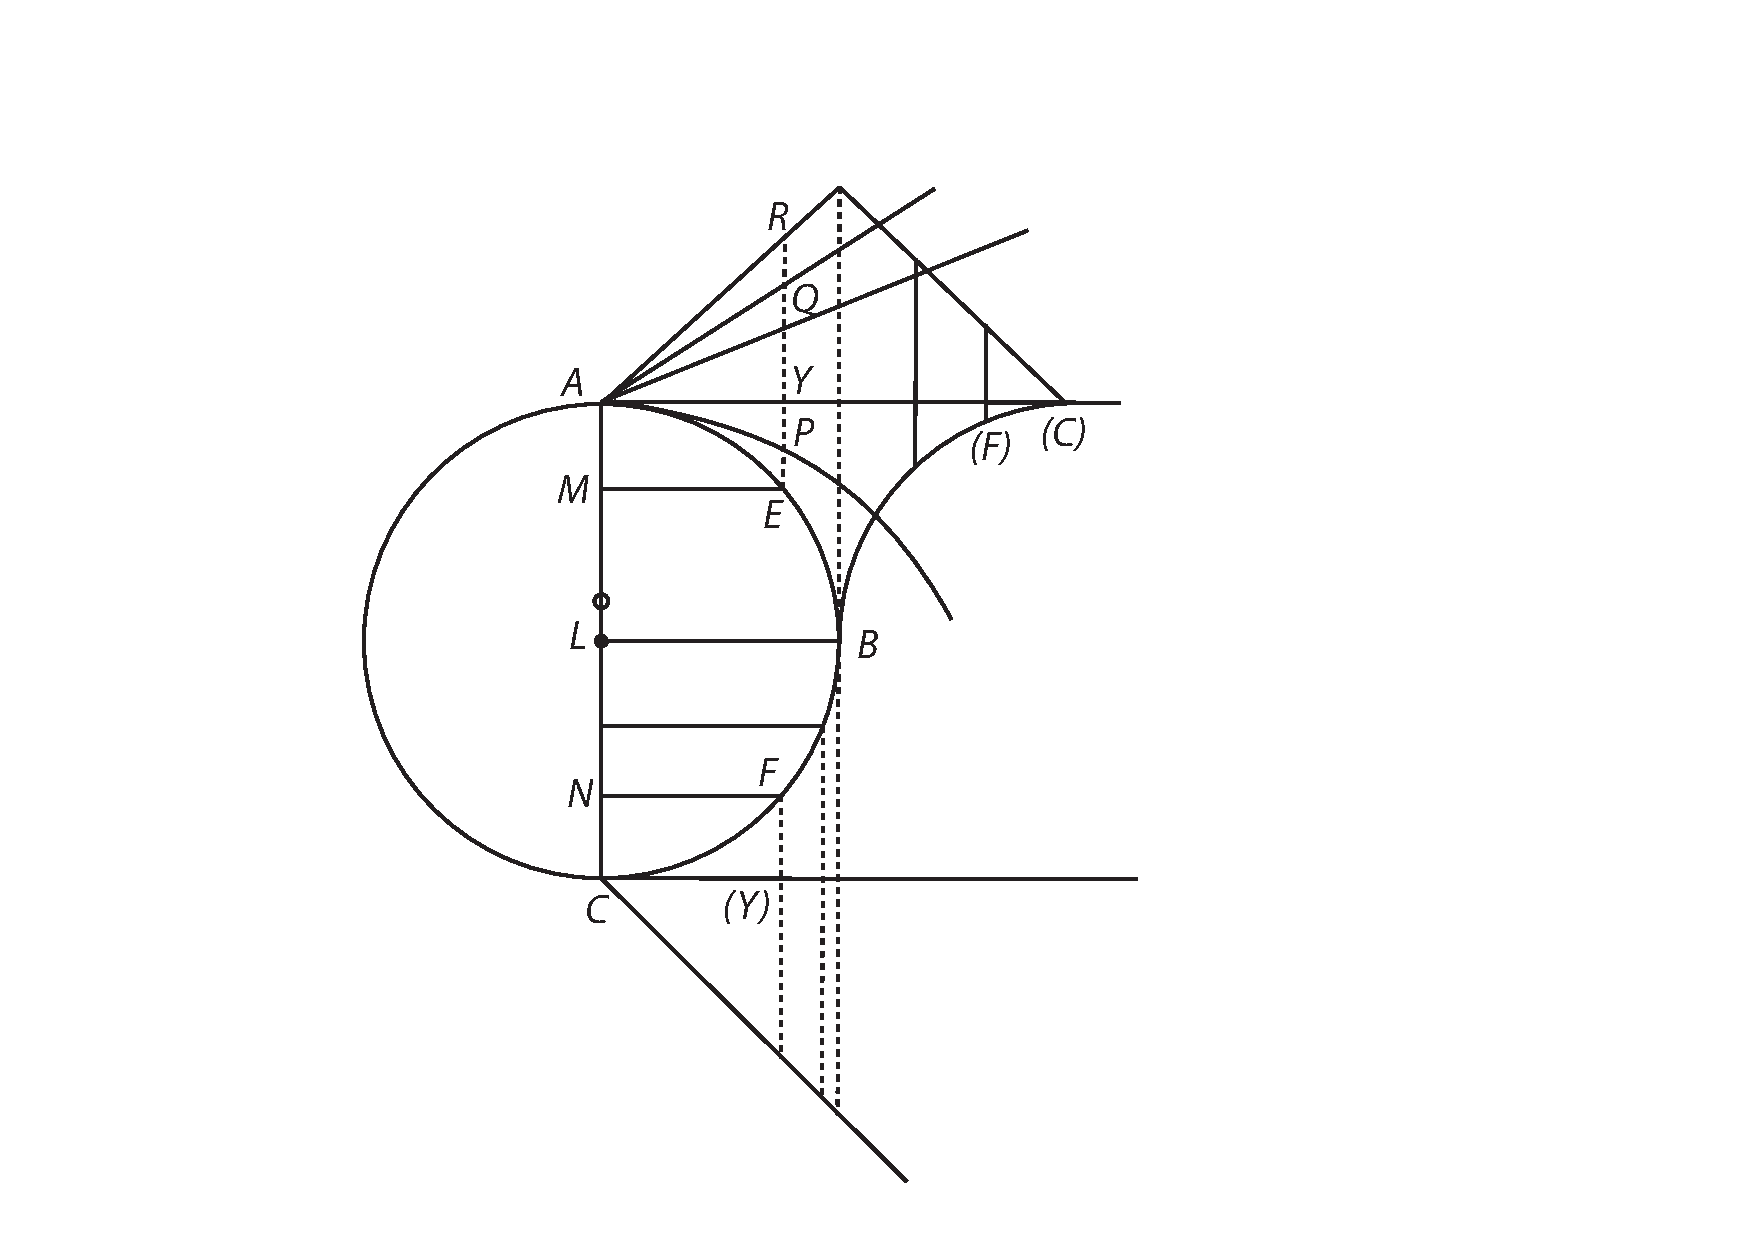
\includegraphics[width=1.0\textwidth]{images/lh0351009_004r-d2.pdf}
%\noindent \centering [\textit{Fig. 2}]
\end{minipage}
\vspace*{1em}
\hspace*{15mm} [\textit{Fig. 1}]\hspace*{70mm} [\textit{Fig. 2}]
\newpage
\count\Bfootins=1200
\pstart
 \noindent \edtext{simplices}{\lemma{}\Bfootnote{simplices \textit{erg. L}}} in quolibet loco; ordinatae erunt ut vires machinae\protect\index{Sachverzeichnis}{vires machinae} ex \edtext{acceleratione\protect\index{Sachverzeichnis}{acceleratio}, in}{\lemma{}\Bfootnote{acceleratione \textbar\ factae \textit{gestr.} \textbar\ , in \textit{L}}} quolibet loco, quippe harum differentiarum \edtext{summae. Aliter si sit figura}{\lemma{summae.}\Bfootnote{\textit{(1)} Aliter describatur figura omnium \textit{(2)} Aliter si sit figura \textit{L}}} cujus ordinatae sint ut $FG. HI. KB$ homogenea illis scilicet, cylinder\protect\index{Sachverzeichnis}{cylinder} ipsarum $LB$, exhibebit vires acceleratas\protect\index{Sachverzeichnis}{vis accelerata}, nempe rectangulum sub $LB$, et recta constante velut $A$. 
\pend
%\begin{figure}[t]
%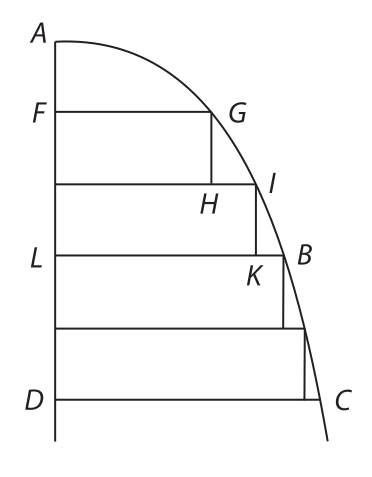
\includegraphics[width=0.2\textwidth]{images/lh0351009_004r-d1.pdf}\hspace{5mm}
%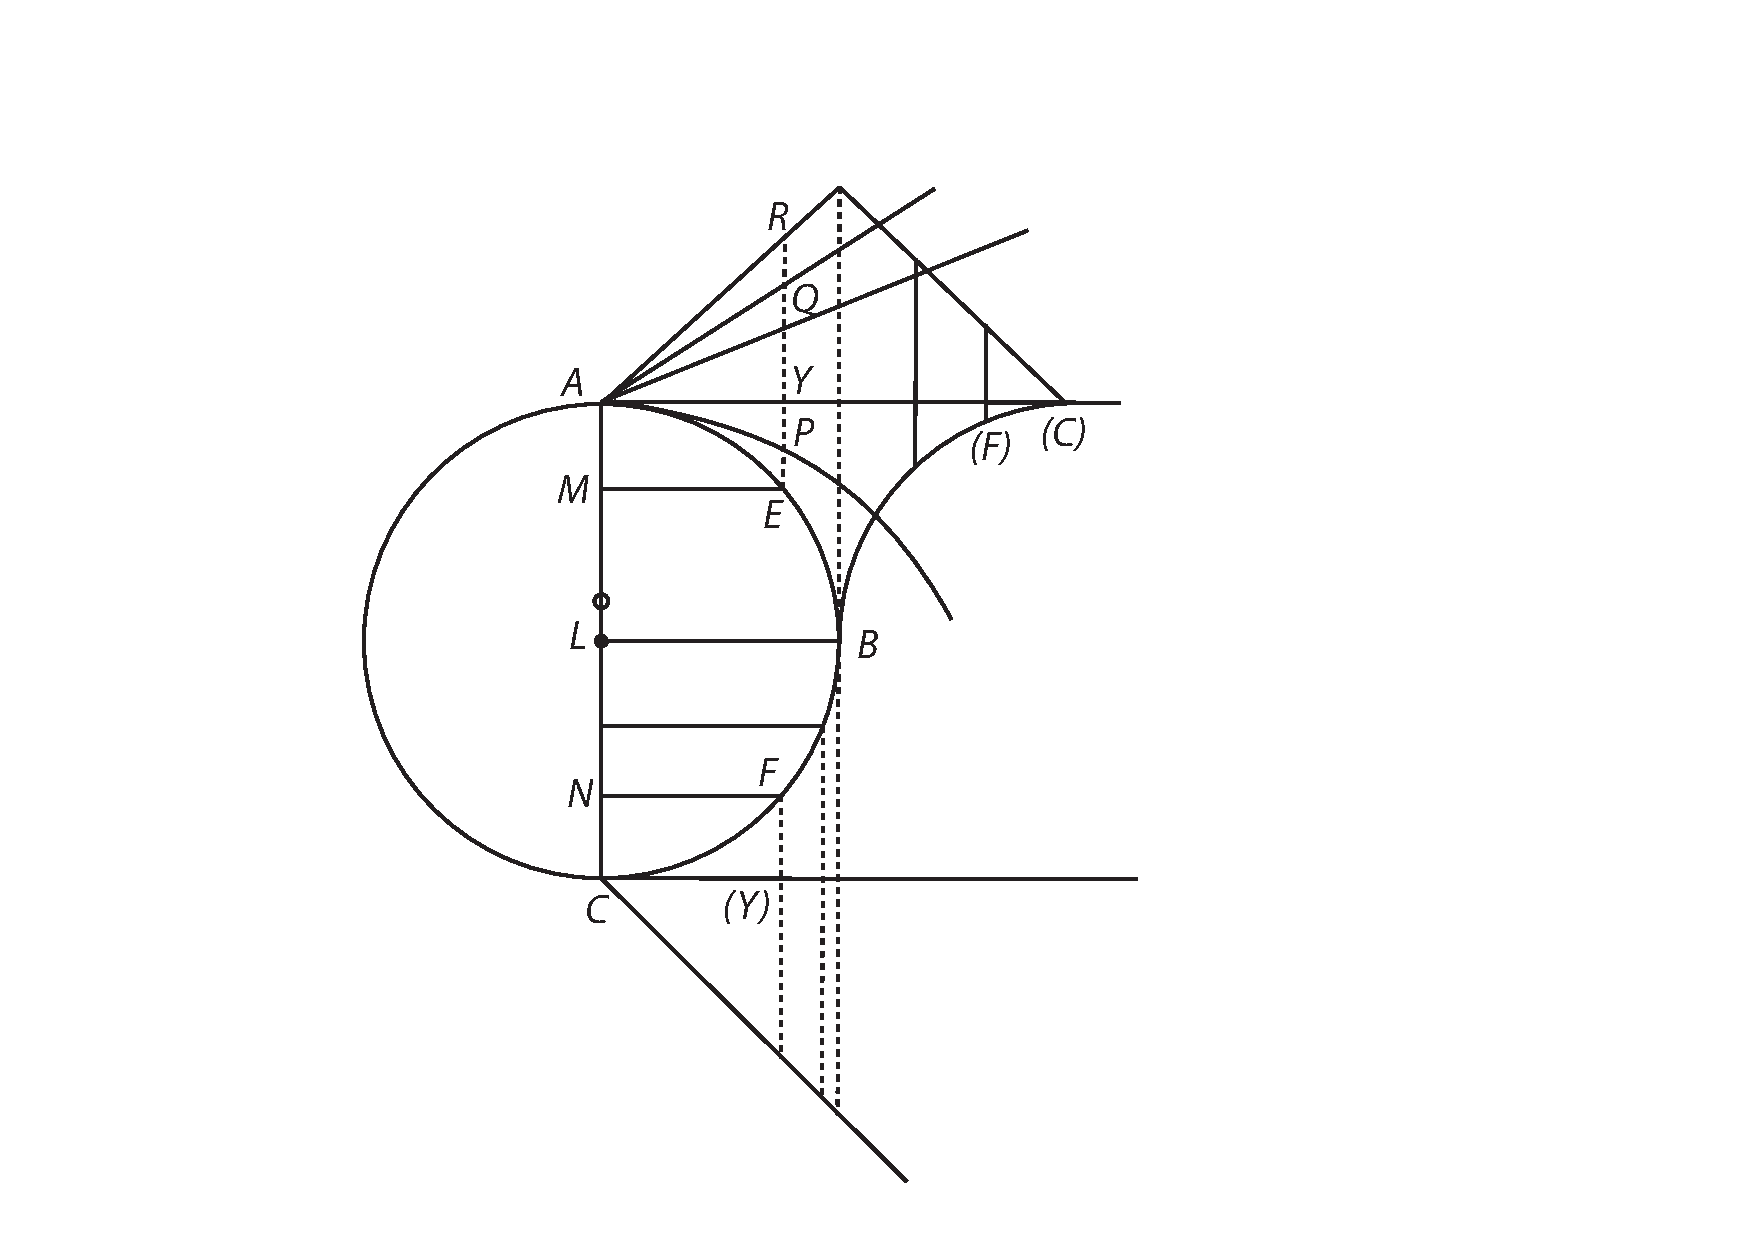
\includegraphics[width=0.4\textwidth]{images/lh0351009_004r-d2.pdf}\\
%\hspace{15mm} [\textit{Fig. 1}] \hspace{35mm} [\textit{Fig. 2}]
%\end{figure}
\pstart Centro $L$ ut ante sit idem circulus $AE$ in tangente verticis $A$, sume $AY$, quamlibet aequalem cuilibet $EM \hspace{0.1mm} \sqcap  \hspace{0.1mm}y$. Cui applicabis \edtext{$YR \hspace{0.1mm} \sqcap \hspace{0.1mm}y$}{\lemma{applicabis}\Bfootnote{\textit{(1)} $YR \sqcap \displaystyle\frac{a}{b}$ \textit{(2)} $ YR \sqcap y$ \textit{L}}} ab uno latere, quae sunt ad lineam rectam $AR$, et \edtext{$YE \sqcap AM \sqcap \sqrt{a^2-y^2}$}{\lemma{et}\Bfootnote{\textit{(1)} ${\displaystyle\frac{b \sqrt{a^2 - y^2}}{a}}$ \textit{(2)} $YE \sqcap AM \sqcap \sqrt{a^2-y^2}$ \textit{L}}} ab altero latere, quae sunt ad circumferentiam $AEB$, ab $AR$, aufer $RQ \sqcap \displaystyle\frac{yb}{a}$\rule[-4mm]{0pt}{10mm} quae sunt etiam ad lineam \edtext{rectam et ab $YE$}{\lemma{rectam}\Bfootnote{\textit{(1)} et $AR$ \textit{(2)} et ab $YE$ \textit{L}}} aufer $PE \sqcap b \sqrt{a^2-y^2}$ quae est ad Ellipsin, residua figura erit summa omnium virium seu quantitas \edtext{acceleratione\protect\index{Sachverzeichnis}{acceleratio} quaesita}{\lemma{acceleratione}\Bfootnote{\textit{(1)} genita \textit{(2)} quaesita \textit{L}}}. Porro pro $NF$, et aliis infra $LB$, eas applicabimus ad [$C(Y)$]\edtext{}{\Bfootnote{$CY$\textit{\ L \"{a}ndert Hrsg.}}}. Nisi malimus arcum $BFC$ illuc transferre in $B(F)(C)$, ut una inde fiat figura continua. His ergo intellectis breviter regulam ita concipiemus: 
\pend 
%\vspace{2mm}
\begin{center}                   
\noindent 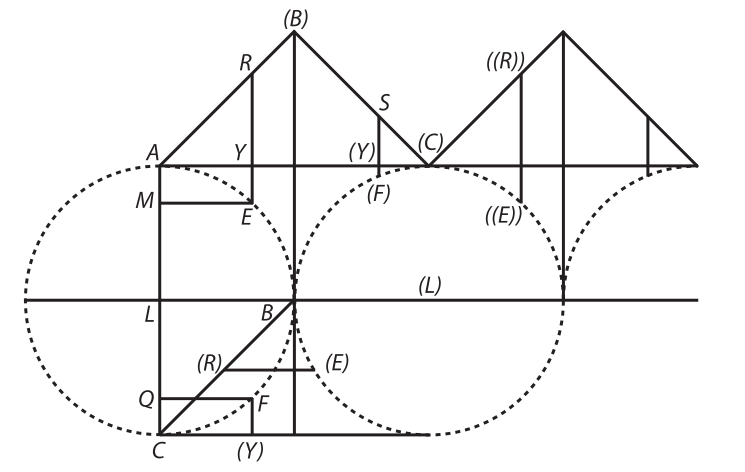
\includegraphics[width=0.86\textwidth]{images/lh0351009_004r-d3.pdf}\newline
[\textit{Fig. 3}]
\end{center}
\count\Bfootins=1200
\pstart Circuli $L\ AEBC$ rotam repraesentantis, verticem recta tangens $AY(C)$ producatur indefinite. Quemadmodum et diameter ejusdem horizonti parallela, $LB$ in qua sumta $(L)B \sqcap LB$ centro $L$, radio $LB$ describatur alius \edtext{circulus $(L)B(C)$}{\lemma{circulus}\Bfootnote{\textit{(1)} $L(B)C$ \textit{(2)} $(L)B(C)$ \textit{L}}} priori aequalis. Ex $B$ erigatur $B(B)$ ipsi $LB$ sive horizonti perpendicularis, et aequalis $AC$ circuli diametro, jungantur $A(B)$, $(B)(C)$. Et spatium \edtext{[$A(B)(C)(F)BE$]}{\lemma{}\Bfootnote{$A(B)(C)FBE$\textit{\ L \"{a}ndert Hrsg.}}} duobus circumferentiae quadrantibus $AEB$ et \textso{$B(F)(C)$} duabusque rectis \edtext{$A(B)$ et $(B)(C)$}{\lemma{}\Bfootnote{$A(B)$ et $(B)(C)$ \textit{erg. L}}} angulum comprehendentibus rectum, contentum erit accelerationibus\protect\index{Sachverzeichnis}{acceleratio} seu viribus crescentibus\protect\index{Sachverzeichnis}{vires crescentes} homogeneum. Nimirum pone motum incipere \edtext{in $E$, nempe $AC$ extremo diametri solidae in $E$, prius}{\lemma{incipere}\Bfootnote{\textit{(1)} $A$ in extremo diametri solidae in $E$, \textit{(2)} in $E$ nempe [...] $E$, prius \textit{L}}} translato, et quaeri quanta sit vis acquisita machinae in \edtext{quodam}{\lemma{}\Bfootnote{quodam \textit{erg. L}}} puncto, v.g. $F$, ad vim\protect\index{Sachverzeichnis}{vis} quaesitam in alio puncto \edtext{v.g. $B$. Ducatur recta $ER$ parallela ipsi $B(B)$, arcui pariter $AEB$, et rectae $A(B)$ occurrens. Inde in quadrante $B(C)$ sumto arcu $B(F)$ aequali}{\lemma{v.g. $B$.}\Bfootnote{\textit{(1)} Sume arcum \textit{(2)} Ducatur recta \textit{ER} parallela \textbar\ ipsi \textit{erg.} \textbar\ $B(B)$, [...] Inde \textit{(a)} sumto arcu $BF$ \textit{(b)} in quadrante [...] aequali \textit{L}}} arcui $BF$ ducatur eodem modo recta [$(F)S$]\edtext{}{\Bfootnote{$FS$\textit{\ L \"{a}ndert Hrsg.}}}, eritque vis acquisita in $F$ ad vim acquisitam\protect\index{Sachverzeichnis}{vis acquisita} in $B$, ut spatium $ER(B)BE$, ad spatium $ER(B)S(F)BE$. Unde apparet si nulla vi extrinseca\protect\index{Sachverzeichnis}{vis extrinseca} accedente repeti fingatur circulatio etiam figuram $A(B)(C)(F)BE$, repetendam, et si exempli causa repetita circulatione rursus pervenerit in $E$ vim acquisitam\protect\index{Sachverzeichnis}{vis acquisita} fore ut spatium $ER(B)(C)(F)BE + ((E))((R))(C)((E))$ id est si motus in $E$ incepisse intelligatur ut spatium $A(B)(C)(F)BE$. Nam si motus in $A$ coepisset, foret ut $A(B)(C)(F)BE + ((E))((R))(C)((E))$ quorum facilis ex superioribus demonstratio est nam si superiores vires simplices\protect\index{Sachverzeichnis}{vis simplex} dividantur per constantem quantitatem omnibus communem, \rule[-4mm]{0pt}{10mm}$\displaystyle \frac{a-b}{ba}$ restabit: $ y + \sqrt{a^2-y^2} \sqcap ER$ quia $ EY \sqcap AM \sqcap \sqrt{a^2-y^2}$ et $YR \sqcap AY \sqcap ME \sqcap y$ quod idem in aliis punctis omnibus obtinet.
\pend 
\pstart \edtext{Sed in machina praesente}{\lemma{Sed}\Bfootnote{\textit{(1)} id quidem \textit{(2)} in machina praesente \textit{L}}} figurae $\aleph$ motu semel in $A$, vel inter $A$ et $B$ coepto. Descensus infra $B$ aestimari non debet; nam inspecta dicta figura $\aleph$. $LE$ diametro rotae solido translato in $LB$ et $LH$ in $LA$ pondus $I$ transibit in $A$, et $LF$ eodem tempore in $C$ translato pondus $F$ assurget versus $L$, verbo redibit status primus $ABCD$.
\pend 
\count\Bfootins=1500
\pstart Pour estimer la force\protect\index{Sachverzeichnis}{force} de la m\^{e}me machine gagn\'{e}e par l'acceleration\protect\index{Sachverzeichnis}{acceleration}; du centre L, et du rayon $LA$ pris \`{a} discretion soit d\'{e}crit le quart de cercle, $LAEB$, le quel soit continu\'{e} mais d'une maniere renvers\'{e}e en forme de serpentine ou 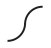
\includegraphics[width=0.035\textwidth]{images/lh0351009_004r-d6.pdf} (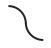
\includegraphics[width=0.035\textwidth]{images/lh0351009_004r-d7.pdf}) en $B(E)(B)$ et cette \makebox[1.0\textwidth][s]{continuation renvers\'{e}e sera repet\'{e}e autant de fois, que la roue de la Machine propos\'{e}e}
\pend
\begin{center}                    
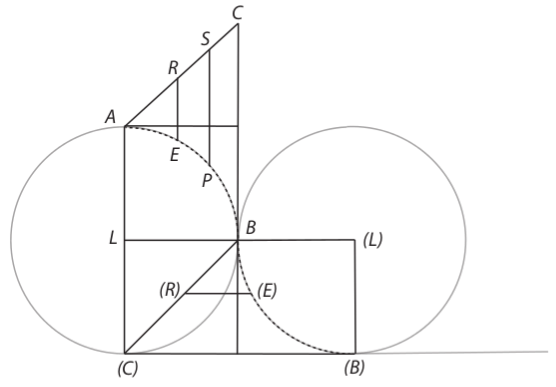
\includegraphics[width=0.8\textwidth]{images/lh0351009_004r-d4.pdf}\\
\hspace{20mm}[\textit{Fig. 4}]
\end{center}
\count\Bfootins=1200
\pstart
\noindent achevera \setline{1}un quart de son tour. \edtext{Soit $BC$, double de $AL$ et parallele \`{a} la m\^{e}me men\'{e}e}{\lemma{Soit $BC$,}\Bfootnote{\textit{(1)} men\'{e}e parall\`{e}le \`{a} $AL$, dont elle soit le double \textit{(2)} double [...] men\'{e}e \textit{L}}} du cost\'{e} de $A$. Joignez $AC$ de m\^{e}me joignez $B(C)$ supposant $AL(C)$ et $(B)(C)$ egales entre elles et \`{a} $BC$. 
\pend
\pstart Or supposons que dans la fig. $\aleph$, le poids \edtext{superieur $E$ \`{a} main droite ou celuy qui luy succedera soit}{\lemma{}\Bfootnote{\`{a} main [...] succedera \textit{erg. L}}} dans le \edtext{point $E$ ou $P$ de la}{\lemma{point $E$}\Bfootnote{\textbar\ ou $P$ \textit{erg.} \textbar\ de la \textit{L}}} dite \edtext{figure $\aleph$ r\'{e}pondant au point $E$ ou $P$}{\lemma{figure $\aleph$}\Bfootnote{\textit{(1)} semblable ou proportionel \`{a} l'arc $AC$ \textit{(2)} r\'{e}pondant au point $E$ ou $P$ \textit{L}}} de la figure \edtext{presente, ou qu'il vienne dans la revolution ou repetition seconde, au}{\lemma{presente, ou}\Bfootnote{\textit{(1)} que dans la seconde \textit{(2)} qu'il \textit{(a)} soit \textit{(b)} vienne [...] seconde, \textit{(aa)} dans le \textit{(bb)} au \textit{L}}} poinct $(E)$ \edtext{de la figure $\aleph$}{\lemma{}\Bfootnote{de la figure $\aleph$ \textit{erg. L}}} qui repond au point $(E)$ de la figure presente. Du point $E$ ou $P$, ou $(E)$ soyent \edtext{[men\'{e}es]}{\lemma{}\Bfootnote{men\'{e}e \textit{L \"{a}ndert Hrsg.}}} sur $AC$, ou $B(C)$ les droites \edtext{ou ordonn\'{e}es}{\lemma{ou ordonn\'{e}es}\Bfootnote{\textit{erg. L}}} $ER$ ou $PS$, ou $(E)(R)$ paralleles \`{a} $BC$ ou $(B)(C)$. Et soit le \edtext{point $A$ ou $E$ celuy du}{\lemma{point}\Bfootnote{\textit{(1)} $E$ \textit{(2)} $A$ ou $E$ celuy du \textit{ L}}} commencement du mouuement\protect\index{Sachverzeichnis}{mouvement}, et celuy du \edtext{point $E$, ou $P$ ou $(E)$}{\lemma{point $E$,}\Bfootnote{\textbar\ ou \textit{erg.} \textbar\ $P$ ou $(E)$ \textit{L}}} celuy de la fin \edtext{dans le temps que nous le considerons}{\lemma{}\Bfootnote{dans [...] considerons \textit{erg. L}}}, je dis que les forces acquises\protect\index{Sachverzeichnis}{force acquise} sur la fin d'un chacun, seront entre elles comme les espaces compris entre les paralleles \edtext{ou ordonn\'{e}es}{\lemma{}\Bfootnote{ou ordonn\'{e}es \textit{erg. L}}} des points du commencement et de la fin. Par exemple si le mouuement\protect\index{Sachverzeichnis}{mouvement} a commenc\'{e} en $A$, la force de la machine\protect\index{Sachverzeichnis}{force de la machine}, acquise par l'acceleration\protect\index{Sachverzeichnis}{acceleration} pendant le poids superieur est en $E$, est \`{a} celle qui est \`{a} acquerir quand il sera en $P$, comme \edtext{l'espace}{\lemma{comme}\Bfootnote{\textit{(1)} les espaces \textit{(2)} l'espace \textit{L}}} $AREA$ compris entre \edtext{le point}{\lemma{}\Bfootnote{le point \textit{erg. L}}} $A$ ou ordonn\'{e}e du commencement infiniment petite, et $ER$ ordonn\'{e}e de la fin; \`{a} l'espace $ASPA$, compris entre $A$ et $PS$. De m\^{e}me la force\protect\index{Sachverzeichnis}{force gagn\'{e}e} gagn\'{e}e par le mouuement commenc\'{e} en $A$ et termin\'{e} en $E$, sera \`{a} la force gagn\'{e}e\protect\index{Sachverzeichnis}{force gagn\'{e}e} par le mouuement commenc\'{e} en $E$, et termin\'{e} en $P$, comme l'espace $AREA$ \`{a} l'espace $ERSPE$. Enfin la force \edtext{gagn\'{e}e\protect\index{Sachverzeichnis}{force gagn\'{e}e} dans}{\lemma{gagn\'{e}e}\Bfootnote{\textit{(1)} par \textit{(1)} dans \textit{L}}} une revolution \edtext{qui se fait pendant que le poids $E$ acheve le quart de cercle}{\lemma{revolution}\Bfootnote{ \textit{ (1) } (c'est \`{a} dire dans un tour du quart de cercle \textit{ (2) } qui [...] cercle \textit{ L}}} $AB$, sera \`{a} la force gagn\'{e}e\protect\index{Sachverzeichnis}{force gagn\'{e}e} dans une revolution et quelque chose d'avantage quand le poids superieur \`{a} main droite est \edtext{en $(E)$ sera comme}{\lemma{en $(E)$}\Bfootnote{\textit{(1)} sera \textit{(2)} comme \textit{L}}} l'espace $ACBA$, compris entre $A$ et $BC$, \`{a} l'espace [$ACBA + B(R)(E)B$]\edtext{}{\Bfootnote{$ACBA + BR(E)B$ \textit{L \"{a}ndert Hrsg.}}} compris entre l'ordonn\'{e}e du \edtext{commencement, s\c{c}avoir le point $A$ (dans cet exemple) et l'ordonn\'{e}e [$(E)(R)$] du}{\lemma{commencement,}\Bfootnote{\textit{(1)} s\c{c}avoir en cet \textit{(2)} s\c{c}avoir [...] \textbar\ $(E)R$ \textit{\"{a}ndert Hrsg.} \textbar\ du \textit{L}}} point de la fin $(E)$. 
\pend 
\count\Bfootins=1000
\pstart Il s'ensuit par l\`{a} que la vistesse croistra \`{a} l'infini, supposant le mouuement continuel, et faisant abstraction des obstacles qui peuuent se rencontrer dans le \edtext{medium; qui est l'air, et l'essieu\protect\index{Sachverzeichnis}{essieu}}{\lemma{medium;}\Bfootnote{\textit{(1)} et dans le poi \textit{(2)} qui est l'air, et l'essieu\protect\index{Sachverzeichnis}{essieu} \textit{L}}} \`{a} l'entour du quel tourne la roue. Car la vitesse\protect\index{Sachverzeichnis}{vitesse} pourroit devenir si grande, que ny l'essieu\protect\index{Sachverzeichnis}{essieu} ny l'air souffriroient l'un un glissement, l'autre une division si subite. Effectivement, si la machine se peut executer, elle viendra bien tost \`{a} une \edtext{vitesse\protect\index{Sachverzeichnis}{vitesse} tres considerable}{\lemma{vitesse}\Bfootnote{\textit{(1)} si grande \textit{(2)} tres considerable \textit{L}}}. Mais \edtext{il faut tacher}{\lemma{il}\Bfootnote{\textit{(1)} faut prendre garde \textit{(2)} faut tacher \textit{L}}} de faire en sorte \edtext{qu'elle devienne}{\lemma{qu'elle}\Bfootnote{\textit{(1)} puisse \textit{(2)} devienne \textit{L}}} jamais plus grande que celle avec la quelle l'aimant attire l'aiguille\protect\index{Sachverzeichnis}{aiguille}. C'est \`{a} dire qu'elle n'acheve pas le quart de cercle avant que l'aimant puisse retirer l'aiguille\protect\index{Sachverzeichnis}{aiguille}. Car cela \edtext{feroit cesser le mouuement en certains cas}{\lemma{feroit}\Bfootnote{\textit{(1)} culbuter la machine. C'est \`{a} dire cela la pourroit mettre en estat de cesser en certains cas \textit{(2)} cesser \textit{(a)} la ma \textit{(b)} le mouuement en certains cas. \textit{L}}}.
\pend
\count\Bfootins=1000
\pstart Il est vray que pendant que l'aiguille\protect\index{Sachverzeichnis}{aiguille} passe sans estre attir\'{e}e, l'acceleration\protect\index{Sachverzeichnis}{acceleration} seroit en m\^{e}me \edtext{temps decroissante}{\lemma{temps}\Bfootnote{\textit{(1)} croissante \textit{(2)} decroissante \textit{L}}}; le mouuement n'estant continu\'{e} par la force gagn\'{e}e\protect\index{Sachverzeichnis}{force gagn\'{e}e}, la quelle, n'estant plus suivie, se perdroit \edtext{peu \`{a} peu}{\lemma{}\Bfootnote{peu \`{a} peu \textit{erg. L}}} par l'obstacle du poids de l'aiguille\protect\index{Sachverzeichnis}{aiguille} \'{e}loign\'{e}e du centre plus qu'il ne faut; \edtext{ce qui peut estre matiere d'un calcul tres subtil}{\lemma{}\Bfootnote{ce qui [...] subtil. \textit{erg. L}}}. Mais l'acceleration\protect\index{Sachverzeichnis}{acceleration} de la force gagn\'{e}e\protect\index{Sachverzeichnis}{force gagn\'{e}e} pourroit estre si grande qu'elle ne donneroit point le loisir \`{a} la machine de se reconnoistre; et qu'elle emporteroit le canal de verre de l'aiguille\protect\index{Sachverzeichnis}{aiguille} qui deuuoit estre \edtext{[attir\'{e}e]}{\lemma{}\Bfootnote{attireroit\textit{\ L \"{a}ndert Hrsg.}}}, et le feroit passer jusque en haut, ou jusque en bas; o\`{u} les aiguilles\protect\index{Sachverzeichnis}{aiguille} demeureroient sans estre attir\'{e}es; et la machine demeureroit en repos; \`{a} moins que la force gagn\'{e}e\protect\index{Sachverzeichnis}{force gagn\'{e}e} fut capable toute seule de porter la machine jusqu' au deuxiesme tour de \edtext{roue dont le mouuement soit assez}{\lemma{roue}\Bfootnote{\textit{(1)} de la vistesse fut asse \textit{(2)} dont le mouuement \textit{(a)} fut \textit{(b)} soit assez \textit{L}}} doux \edtext{pour}{\lemma{}\Bfootnote{pour \textit{erg.} \textit{L}}} attendre l'action de l'aimant. 
\pend 
\vspace{-1mm}
\pstart
\begin{window}[0,r,\hspace{1mm}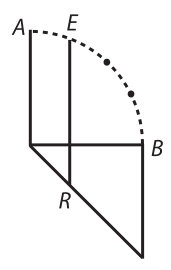
\includegraphics[%trim = -3mm -2mm 0mm 0mm, clip,
width=0.2\textwidth]
{images/lh0351009_004r-d5.pdf}, \hspace{7mm}{[\textit{Fig. 5}]}]
\indent
\edtext{Sed video jam me errasse, nam pro sinubus complementi $\sqrt{a^2-y^2}$ ut $LM$ applicavi sinus versos ut $AM$. Itaque $ER$ esse debebit, qualem in hac novissima figura vides. Succurrunt praeterea difficultates ingentes}{\lemma{7-10\hspace{1.8mm}}\killnumber\Bfootnote{Sed \textbar\ occurrunt \textit{streicht Hrsg.} \textbar\ \textit{(1)} hic duae difficultates ingentes, una an non potius sinus recti et ver \textit{(2)} video [...] $ \sqrt{a^2-y^2}$ \textbar\ ut $LM$ \textit{erg.} \textbar\ applicavi [...] ingentes \textit{L}}}. {Quarum\reversemarginpar\marginnote{\scriptsize\hspace{-13mm}10}} prima est an non ipsae $ER$ potius arcui $AEB$, sive in rectam extenso applicari in plano, sive manenti qualis est in superficie cylindrica insistere debeant. Idque rationi consentaneum magis, quia mobile percurrit curvam circularem $AEB$, et in quolibet arcu summam habet virium\protect\index{Sachverzeichnis}{vis} praecedentium omnium. Suppone autem arcum {divisum\reversemarginpar\marginnote{\scriptsize\hspace{-13mm}15}} in partes infinite parvas inter se aequales. Sed jam hanc quoque methodum [4~v\textsuperscript{o}] habeo suspectam \edtext{falsitatis. Equidem}{\lemma{16 \hspace{1.8mm}falsitatis.}\killnumber\Bfootnote{\textit{(1)} Nam \textit{(2)} Equidem \textit{L}}} supponendo\hspace{0.2mm} infinitos\hspace{0.3mm} istos\hspace{0.3mm} arcus\hspace{0.2mm} lineis\hspace{0.3mm} rectis\hspace{0.3mm} aequales.\hspace{0.3mm} Sit \hspace{0.2mm}\edtext{centro \textit{H}}{\lemma{17\hspace{1.8mm}}\killnumber\Bfootnote{centro \textit{H} \textit{erg. L}}}
\end{window}
%\begin{wrapfigure}[12]{l}{0.2\textwidth}                    
%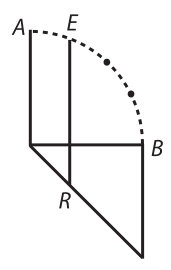
\includegraphics[trim = 0mm -3mm -5mm 0mm, clip, width=0.2\textwidth]{images/lh0351009_004r-d5.pdf}\newline
%\noindent \centering [\textit{Fig. 5}]
%\end{wrapfigure}
%\edtext{Sed video jam me errasse, nam pro sinubus complementi $\sqrt{a^2-y^2}$ ut $LM$ applicavi sinus versos ut $AM$. Itaque $ER$ esse debebit, qualem in hac novissima figura vides. Succurrunt praeterea difficultates ingentes}{\lemma{}\Bfootnote{Sed \textbar\ occurrunt \textit{streicht Hrsg.} \textbar\ \textit{(1)} hic duae difficultates ingentes, una an non potius sinus recti et ver \textit{(2)} video [...] $ \sqrt{a^2-y^2}$ \textbar\ ut $LM$ \textit{erg.} \textbar\ applicavi [...] ingentes \textit{L}}}. Quarum prima est an non ipsae $ER$ potius arcui $AEB$, sive in rectam extenso applicari in plano, sive manenti qualis est in superficie cylindrica insistere debeant. Idque rationi consentaneum magis, quia mobile percurrit curvam circularem $AEB$, et in quolibet arcu summam habet virium\protect\index{Sachverzeichnis}{vis} praecedentium omnium. Suppone autem arcum divisum in partes infinite parvas inter se aequales. Sed jam hanc quoque methodum